% Slides do Trabalho Final - Inteligência Computacional
% Sugestão: usar pacote beamer ou similar

\documentclass[aspectratio=169]{beamer}
\usepackage[utf8]{inputenc}
\usepackage{graphicx}

% Tema moderno para Beamer
\usepackage{lmodern}
\usetheme{metropolis}

\title{Classificação e Regressão Supervisionadas com Algoritmos de Aprendizado de Máquina}
\author{Leonardo Vieira Guimarães \\ Programa de Pós-Graduação em Modelagem Matemática e Computacional, CEFET-MG}
\date{29 de julho de 2025}


\begin{document}

% Capa customizada
{
  \begin{frame}[plain]
    \vspace{0.5cm}
    \centering
    {\usebeamerfont{title}\usebeamercolor[fg]{title}\Huge\textbf{Classificação e Regressão Supervisionadas}}\\[0.5em]
    {\usebeamerfont{subtitle}\usebeamercolor[fg]{subtitle}\Large\textit{com Algoritmos de Aprendizado de Máquina}}\\[1.5em]
    \vspace{0.5cm}
    {\usebeamerfont{author}\usebeamercolor[fg]{author}\large Leonardo Vieira Guimarães}\\[0.5em]
    {\usebeamerfont{institute}\usebeamercolor[fg]{institute}\normalsize Programa de Pós-Graduação em Modelagem Matemática e Computacional, CEFET-MG}\\[1em]
    {\usebeamerfont{date}\usebeamercolor[fg]{date}\normalsize 29 de julho de 2025}
    \vfill
  \end{frame}
}

\begin{frame}{Motivação e Objetivo}
  \begin{itemize}
    \item Inteligência Computacional é fundamental para resolver problemas complexos em ciência de dados, engenharia e saúde.
    \item Necessidade de modelos preditivos robustos e confiáveis diante do aumento de dados.
    \item Objetivo: comparar técnicas de regressão e classificação multiclasse em bases públicas (Energy Efficiency, California Housing, Wine Quality, Iris).
    \item Avaliar modelos lineares, ensembles, redes neurais e métodos baseados em margens, considerando diferentes estratégias de pré-processamento.
  \end{itemize}
\end{frame}

% --- Slide 1: Processamento dos Dados ---
\begin{frame}{Processamento dos Dados}
  \begin{itemize}
   \item Datasets utilizados:
    \begin{itemize}
      \item \textbf{Regressão:} Energy Efficiency, California Housing
      \item \textbf{Classificação:} Wine Quality (Red), Iris
    \end{itemize}
    \item Pré-processamento:
      \begin{itemize}
        \item Normalização dos atributos (para regressão e classificação)
        \item Codificação de variáveis categóricas (quando necessário)
        \item Divisão dos dados em treino e teste:
          \begin{itemize}
            \item Regressão: divisão aleatória (70\% treino, 30\% teste)
            \item Classificação: divisão estratificada (70\% treino, 30\% teste) para preservar a proporção das classes
          \end{itemize}
        \item Balanceamento de classes para classificação: aplicado em Wine Quality e Iris para melhorar a acurácia e F1-score
      \end{itemize}
  \end{itemize}
\end{frame}

% --- Slide: Energy Efficiency Dataset ---
\begin{frame}{Energy Efficiency Dataset}
  \begin{itemize}
    \item \textbf{Tipo:} Regressão
    \item \textbf{Amostras:} 768
    \item \textbf{Atributos:} 8 variáveis de entrada (ex: área, orientação, compactação, etc.)
    \item \textbf{Alvos:} Y1 (Heating Load), Y2 (Cooling Load)
    \item \textbf{Descrição:} Dados de edifícios simulados para prever consumo de energia para aquecimento e resfriamento.
    \item \textbf{Fonte:} UCI Machine Learning Repository
  \end{itemize}
\end{frame}

% --- Slide: California Housing Dataset ---
\begin{frame}{California Housing Dataset}
  \begin{itemize}
    \item \textbf{Tipo:} Regressão
    \item \textbf{Amostras:} 20.640
    \item \textbf{Atributos:} 8 variáveis de entrada (ex: média de quartos, população, latitude, longitude, etc.)
    \item \textbf{Alvo:} MedHouseVal (valor mediano das casas em milhares de dólares)
    \item \textbf{Descrição:} Dados do censo da Califórnia para prever o valor das casas por região.
    \item \textbf{Fonte:} StatLib, UCI Machine Learning Repository
  \end{itemize}
\end{frame}

% --- Slide: Wine Quality (Red) Dataset ---
\begin{frame}{Wine Quality (Red) Dataset}
  \begin{itemize}
    \item \textbf{Tipo:} Classificação multiclasse
    \item \textbf{Amostras:} 1.599
    \item \textbf{Atributos:} 11 variáveis físico-químicas (ex: acidez, açúcar, pH, álcool, etc.)
    \item \textbf{Alvo:} Qualidade do vinho (nota de 3 a 8)
    \item \textbf{Descrição:} Avaliação da qualidade de vinhos tintos portugueses com base em características químicas.
    \item \textbf{Fonte:} UCI Machine Learning Repository
  \end{itemize}
\end{frame}

% --- Slide: Iris Dataset ---
\begin{frame}{Iris Dataset}
  \begin{itemize}
    \item \textbf{Tipo:} Classificação multiclasse
    \item \textbf{Amostras:} 150
    \item \textbf{Atributos:} 4 variáveis (comprimento e largura das sépalas e pétalas)
    \item \textbf{Alvo:} Espécie da flor (Setosa, Versicolor, Virginica)
    \item \textbf{Descrição:} Clássico conjunto de dados para classificação de espécies de íris.
    \item \textbf{Fonte:} UCI Machine Learning Repository
  \end{itemize}
\end{frame}

% --- Slide 2: Métodos de Treinamento ---
\begin{frame}{Métodos de Treinamento}
  \begin{itemize}
    \item Modelos avaliados:
      \begin{itemize}
        \item \textbf{Regressão:} Linear Regression, Random Forest Regressor, MLPRegressor, SVR (Support Vector Regressor)
        \item \textbf{Classificação:} Logistic Regression, Random Forest Classifier, MLPClassifier, SVM (Support Vector Machine)
      \end{itemize}
    \item Cada experimento foi repetido 30 vezes para garantir robustez estatística dos resultados.
  \end{itemize}
\end{frame}

% --- Slide: Modelos Lineares ---
\begin{frame}{Modelos Lineares}
  \begin{itemize}
    \item \textbf{O que são?} Modelos que assumem uma relação linear entre as variáveis de entrada e a saída.
    \item \textbf{Exemplos:} Regressão Linear (para prever valores contínuos) e Regressão Logística (para classificação).
    \item \textbf{Características:}
      \begin{itemize}
        \item Simples, rápidos e fáceis de interpretar.
        \item Funcionam bem quando a relação entre as variáveis é aproximadamente linear.
        \item Limitados para problemas com relações não-lineares complexas.
      \end{itemize}
  \end{itemize}
\end{frame}

% --- Slide: Ensembles (Random Forest) ---
\begin{frame}{Ensembles: Random Forest}
  \begin{itemize}
    \item \textbf{O que são?} Técnicas que combinam vários modelos simples (como árvores de decisão) para formar um modelo mais robusto.
    \item \textbf{Exemplo:} Random Forest, que constrói diversas árvores de decisão e faz a média (regressão) ou votação (classificação) dos resultados.
    \item \textbf{Características:}
      \begin{itemize}
        \item Reduzem o risco de overfitting.
        \item Lidam bem com dados ruidosos e desbalanceados.
        \item Geralmente apresentam alta precisão em problemas reais.
      \end{itemize}
  \end{itemize}
\end{frame}

% --- Slide: Redes Neurais (MLP) ---
\begin{frame}{Redes Neurais: MLP}
  \begin{itemize}
    \item \textbf{O que são?} Modelos inspirados no cérebro humano, compostos por camadas de neurônios artificiais.
    \item \textbf{Exemplo:} MLP (Perceptron Multicamadas), com múltiplas camadas ocultas entre entrada e saída.
    \item \textbf{Características:}
      \begin{itemize}
        \item Capazes de aprender relações não-lineares complexas.
        \item Requerem mais dados e processamento.
        \item Muito flexíveis, mas podem ser difíceis de interpretar.
      \end{itemize}
  \end{itemize}
\end{frame}

% --- Slide: Métodos Baseados em Margens (SVM/SVR) ---
\begin{frame}{Métodos Baseados em Margens: SVM/SVR}
  \begin{itemize}
    \item \textbf{O que são?} Algoritmos que buscam separar as classes (ou ajustar uma faixa para regressão) maximizando a margem entre os dados.
    \item \textbf{Exemplo:} SVM (Support Vector Machine) para classificação e SVR (Support Vector Regressor) para regressão.
    \item \textbf{Características:}
      \begin{itemize}
        \item Eficazes para dados com fronteiras complexas.
        \item Sensíveis à escolha dos parâmetros e à normalização dos dados.
        \item Podem alcançar alta precisão em problemas bem definidos.
      \end{itemize}
  \end{itemize}
\end{frame}


% --- Slide: Acurácia e F1-score ---
\begin{frame}{Métricas de Avaliação: Classificação}
  \begin{itemize}
    \item \textbf{Acurácia:}
      \begin{itemize}
        \item Proporção de acertos sobre o total de previsões.
        \item Fórmula: $\text{Acurácia} = \frac{TP + TN}{TP + TN + FP + FN}$
      \end{itemize}
    \item \textbf{F1-score:}
      \begin{itemize}
        \item Média harmônica entre precisão e revocação.
        \item Fórmula: $F_1 = 2 \cdot \frac{\text{Precis\~ao} \cdot \text{Revoca\c{c}\~ao}}{\text{Precis\~ao} + \text{Revoca\c{c}\~ao}}$
        \item Útil para bases desbalanceadas.
      \end{itemize}
      \item \textbf{Kappa:}
      \begin{itemize}
        \item Mede o acordo entre as previsões do modelo e os valores reais, corrigido pelo acaso.
        \item Fórmula: $Kappa = \frac{p_o - p_e}{1 - p_e}$
        \item $p_o$ = acurácia observada, $p_e$ = acurácia esperada pelo acaso.
      \end{itemize}
  \end{itemize}
\end{frame}

% --- Slide: Matriz de Confusão ---
\begin{frame}{Matriz de Confusão}
  \begin{columns}
    \column{0.6\textwidth}
      \begin{itemize}
        \item Mostra acertos e erros do modelo para cada classe.
        \item Permite identificar:
          \begin{itemize}
            \item \textbf{TP}: Verdadeiro Positivo
            \item \textbf{TN}: Verdadeiro Negativo
            \item \textbf{FP}: Falso Positivo
            \item \textbf{FN}: Falso Negativo
          \end{itemize}
        \item Base para métricas como acurácia, precisão, revocação, F1-score, entre outras.
      \end{itemize}
    \column{0.4\textwidth}
      \centering
      \begin{tabular}{c|cc}
        & P & N \\
        \hline
        P & TP & FN \\
        N & FP & TN \\
      \end{tabular}
  \end{columns}
\end{frame}

% --- Slide: Métricas de Regressão ---
\begin{frame}{Métricas de Avaliação: Regressão}
  \begin{itemize}
    \item \textbf{RMSE (Root Mean Squared Error):}
      \begin{itemize}
        \item Mede o erro quadrático médio entre valores previstos e reais.
        \item Fórmula: $RMSE = \sqrt{\frac{1}{n} \sum_{i=1}^n (y_i - \hat{y}_i)^2}$
        \item Valores menores indicam melhor desempenho.
      \end{itemize}
    \item \textbf{MAE (Mean Absolute Error):}
      \begin{itemize}
        \item Média dos valores absolutos dos erros.
        \item Fórmula: $MAE = \frac{1}{n} \sum_{i=1}^n |y_i - \hat{y}_i|$
        \item Fácil de interpretar, menos sensível a outliers que o RMSE.
      \end{itemize}
    \item \textbf{$R^2$ (Coeficiente de Determinação):}
      \begin{itemize}
        \item Mede a proporção da variância explicada pelo modelo.
        \item Fórmula: $R^2 = 1 - \frac{\sum_{i=1}^n (y_i - \hat{y}_i)^2}{\sum_{i=1}^n (y_i - \bar{y})^2}$
        \item Valores próximos de 1 indicam bom ajuste.
      \end{itemize}
  \end{itemize}
\end{frame}

% --- Slide: Scatter Plot (Regressão) ---
\begin{frame}{Gráfico de Dispersão (Scatter Plot)}
  \begin{columns}
    \column{0.5\textwidth}
      \begin{itemize}
        \item Utilizado para comparar visualmente os valores reais e previstos em problemas de regressão.
        \item Pontos próximos da linha $y = x$ indicam boas previsões.
      \end{itemize}
    \column{0.5\textwidth}
      \centering
      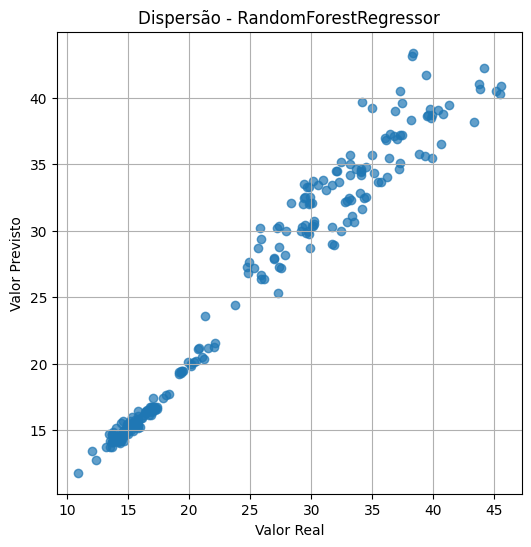
\includegraphics[width=0.9\linewidth]{../graficos/exp_energy_efficiency_y2_RandomForestRegressor.png} % Substitua pelo nome correto do arquivo de imagem
  \end{columns}
\end{frame}

% --- Slide: Energy Efficiency - Regressão Y1 (Resultados) ---
\begin{frame}{Energy Efficiency: Regressão (Y1) - Resultados}
  \begin{itemize}
    \item \textbf{Modelos avaliados:} Linear Regression, Random Forest Regressor, MLPRegressor, SVR
    \item \textbf{Resultados para Y1:}
      \begin{itemize}
        \item \textbf{Linear Regression:} RMSE = 2.9708, MAE = 2.1091, $R^2$ = 0.9128
        \item \textbf{Random Forest:} RMSE = 0.5171, MAE = 0.3450, $R^2$ = 0.9973
        \item \textbf{MLPRegressor:} RMSE = 2.6173, MAE = 1.8412, $R^2$ = 0.9322
        \item \textbf{SVR:} RMSE = 2.8290, MAE = 1.9028, $R^2$ = 0.9210
      \end{itemize}
  \end{itemize}
\end{frame}

% --- Slide: Energy Efficiency - Regressão Y1 (Gráficos de Dispersão) ---
\begin{frame}{Energy Efficiency: Regressão (Y1) - Gráficos de Dispersão}
  \begin{itemize}
    \item \textbf{Análise:} Modelos com pontos mais próximos da diagonal indicam melhores previsões. Random Forest apresenta maior aderência à linha ideal, enquanto Linear Regression e SVR mostram maior dispersão.
  \end{itemize}
  \begin{columns}
    \column{0.25\textwidth}
      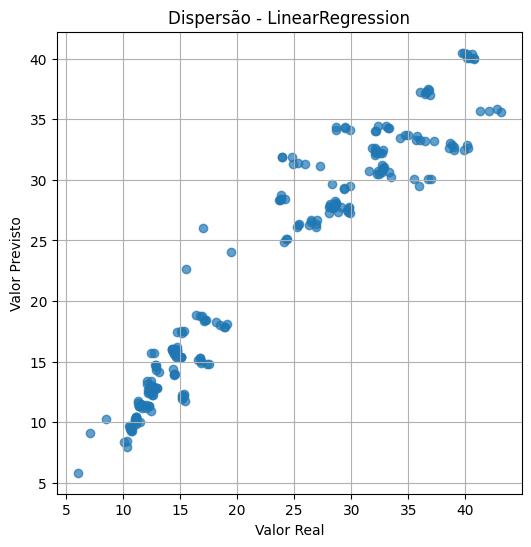
\includegraphics[width=\linewidth]{../graficos/exp_energy_efficiency_y1_LinearRegression.png}
      \centering\scriptsize Linear Regression
    \column{0.25\textwidth}
      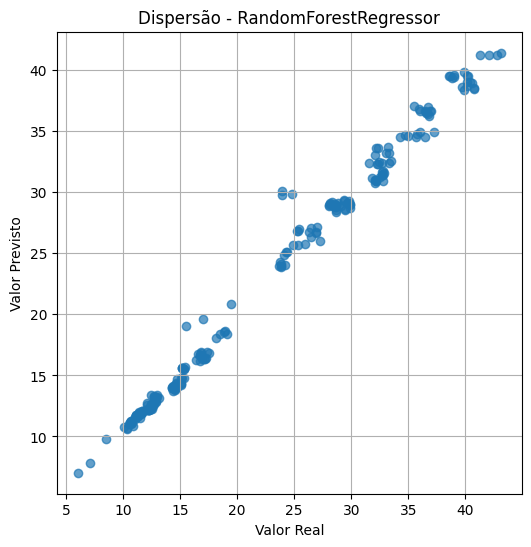
\includegraphics[width=\linewidth]{../graficos/exp_energy_efficiency_y1_RandomForestRegressor.png}
      \centering\scriptsize Random Forest
    \column{0.25\textwidth}
      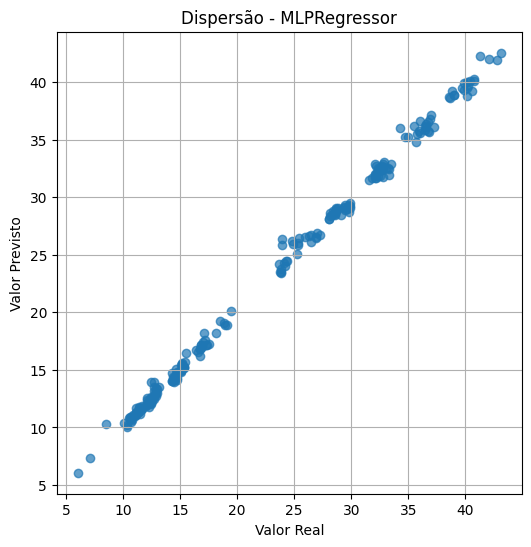
\includegraphics[width=\linewidth]{../graficos/exp_energy_efficiency_y1_MLPRegressor.png}
      \centering\scriptsize MLPRegressor
    \column{0.25\textwidth}
      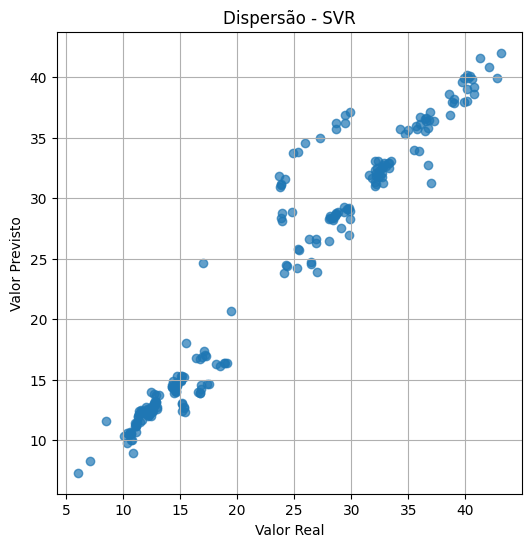
\includegraphics[width=\linewidth]{../graficos/exp_energy_efficiency_y1_SVR.png}
      \centering\scriptsize SVR
  \end{columns}
\end{frame}

% --- Slide: Energy Efficiency - Regressão Y2 (Resultados) ---
\begin{frame}{Energy Efficiency: Regressão (Y2) - Resultados}
  \begin{itemize}
    \item \textbf{Modelos avaliados:} Linear Regression, Random Forest Regressor, MLPRegressor, SVR
    \item \textbf{Resultados para Y2:}
      \begin{itemize}
        \item \textbf{Linear Regression:} RMSE = 3.2059, MAE = 2.2713, $R^2$ = 0.8849
        \item \textbf{Random Forest:} RMSE = 1.7317, MAE = 1.0485, $R^2$ = 0.9663
        \item \textbf{MLPRegressor:} RMSE = 2.9967, MAE = 2.1238, $R^2$ = 0.8993
        \item \textbf{SVR:} RMSE = 3.1696, MAE = 2.1104, $R^2$ = 0.8875
      \end{itemize}
  \end{itemize}
\end{frame}

% --- Slide: Energy Efficiency - Regressão Y2 (Gráficos de Dispersão) ---
\begin{frame}{Energy Efficiency: Regressão (Y2) - Gráficos de Dispersão}
  \begin{itemize}
    \item \textbf{Análise:} Random Forest novamente apresenta maior aderência à linha ideal, indicando melhor desempenho. Linear Regression e SVR mostram maior dispersão dos pontos, sugerindo maior erro nas previsões.
  \end{itemize}
  \begin{columns}
    \column{0.25\textwidth}
      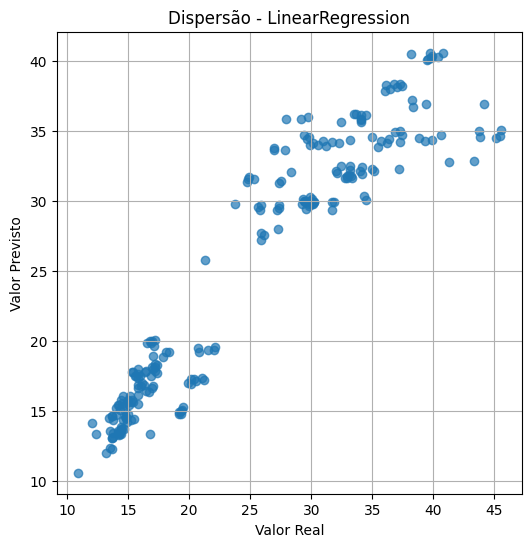
\includegraphics[width=\linewidth]{../graficos/exp_energy_efficiency_y2_LinearRegression.png}
      \centering\scriptsize Linear Regression
    \column{0.25\textwidth}
      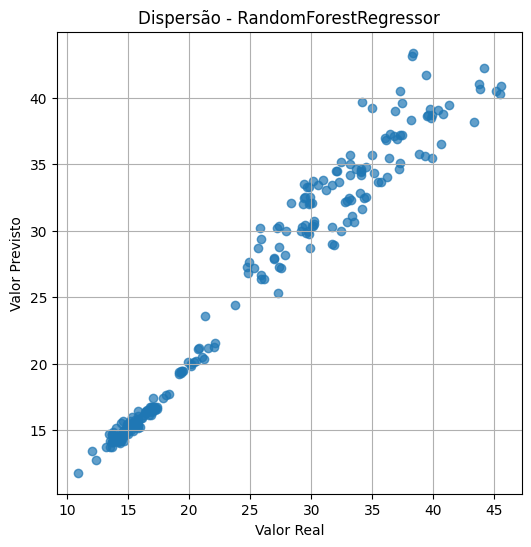
\includegraphics[width=\linewidth]{../graficos/exp_energy_efficiency_y2_RandomForestRegressor.png}
      \centering\scriptsize Random Forest
    \column{0.25\textwidth}
      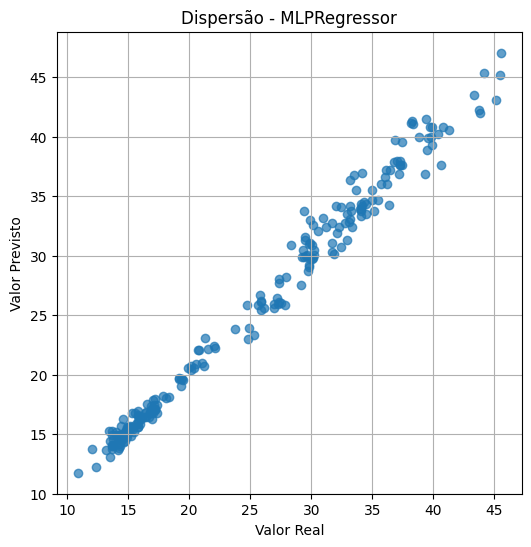
\includegraphics[width=\linewidth]{../graficos/exp_energy_efficiency_y2_MLPRegressor.png}
      \centering\scriptsize MLPRegressor
    \column{0.25\textwidth}
      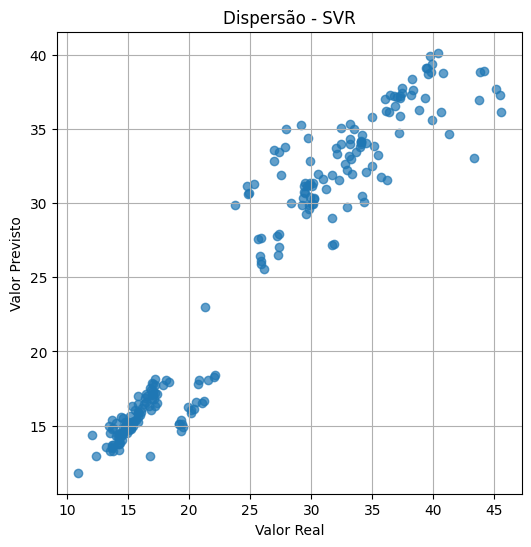
\includegraphics[width=\linewidth]{../graficos/exp_energy_efficiency_y2_SVR.png}
      \centering\scriptsize SVR
  \end{columns}
\end{frame}

% --- Slide: California Housing - Regressão (Resultados) ---
\begin{frame}{California Housing: Regressão - Resultados}
  \begin{itemize}
    \item \textbf{Modelos avaliados:} Linear Regression, Random Forest Regressor, MLPRegressor, SVR
    \item \textbf{Resultados:}
      \begin{itemize}
        \item \textbf{Linear Regression:} RMSE = 0.7361, MAE = 0.5327, $R^2$ = 0.5918
        \item \textbf{Random Forest:} RMSE = 0.5071, MAE = 0.3312, $R^2$ = 0.8069
        \item \textbf{MLPRegressor:} RMSE = 0.5463, MAE = 0.3729, $R^2$ = 0.7757
        \item \textbf{SVR:} RMSE = 0.5925, MAE = 0.3955, $R^2$ = 0.7363
      \end{itemize}
  \end{itemize}
\end{frame}

% --- Slide: California Housing - Regressão (Gráficos de Dispersão) ---
\begin{frame}{California Housing: Regressão - Gráficos de Dispersão}
  \begin{itemize}
    \item \textbf{Análise:} Random Forest apresenta melhor aderência à linha ideal, indicando maior precisão. Linear Regression e SVR mostram maior dispersão dos pontos, sugerindo maior erro nas previsões.
  \end{itemize}
  \begin{columns}
    \column{0.25\textwidth}
      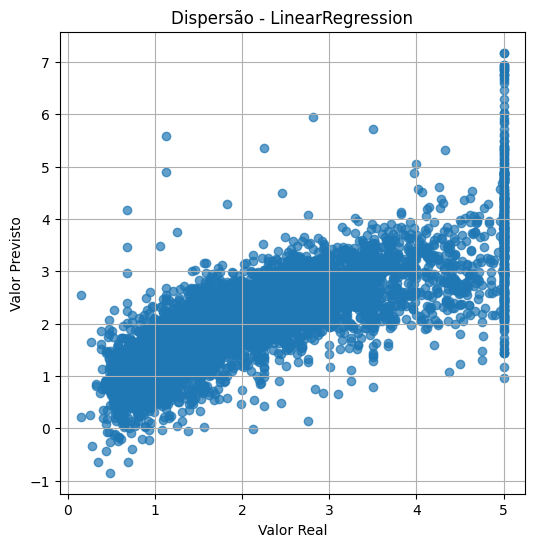
\includegraphics[width=\linewidth]{../graficos/exp_california_housing_LinearRegression.png}
      \centering\scriptsize Linear Regression
    \column{0.25\textwidth}
      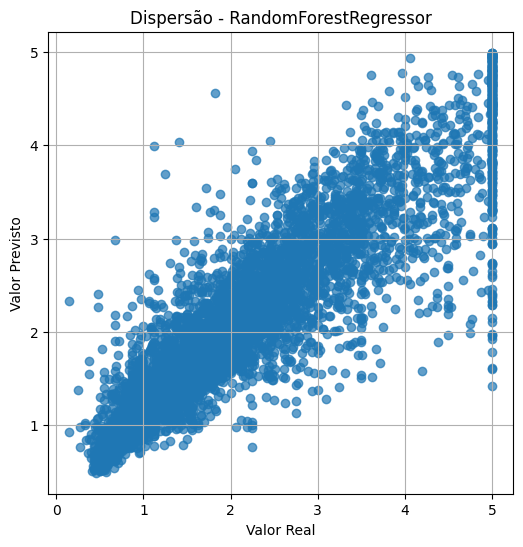
\includegraphics[width=\linewidth]{../graficos/exp_california_housing_RandomForestRegressor.png}
      \centering\scriptsize Random Forest
    \column{0.25\textwidth}
      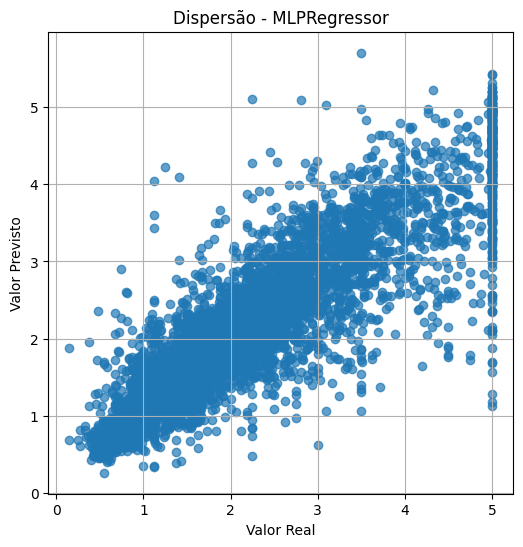
\includegraphics[width=\linewidth]{../graficos/exp_california_housing_MLPRegressor.png}
      \centering\scriptsize MLPRegressor
    \column{0.25\textwidth}
      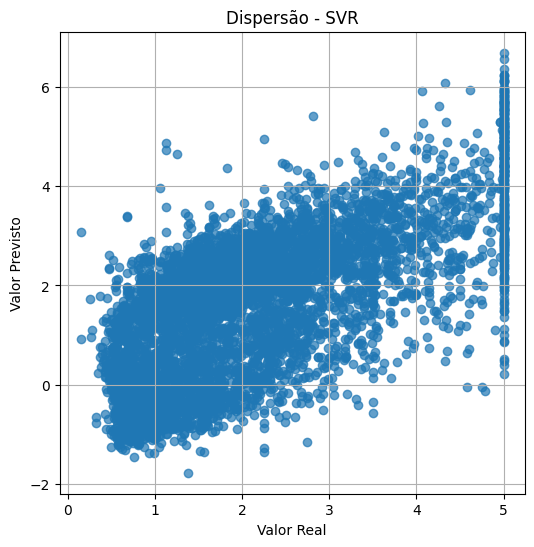
\includegraphics[width=\linewidth]{../graficos/exp_california_housing_SVR.png}
      \centering\scriptsize SVR
  \end{columns}
\end{frame}


% --- Slide: Wine Quality (Red) - Classificação (Resultados) ---
\begin{frame}{Wine Quality (Red): Classificação - Resultados}
  \begin{itemize}
    \item \textbf{Modelos avaliados:} Logistic Regression, Random Forest Classifier, MLPClassifier, SVM
    \item \textbf{Resultados:}
      \begin{itemize}
        \item \textbf{Logistic Regression:} Acurácia = 0.62, F1-score = 0.59, Kappa = 0.47
        \item \textbf{Random Forest:} Acurácia = 0.71, F1-score = 0.70, Kappa = 0.60
        \item \textbf{MLPClassifier:} Acurácia = 0.66, F1-score = 0.64, Kappa = 0.53
        \item \textbf{SVM:} Acurácia = 0.64, F1-score = 0.62, Kappa = 0.50
      \end{itemize}
    \item \textbf{Análise:} Random Forest apresentou o melhor desempenho geral.
  \end{itemize}
\end{frame}

% --- Slide: Wine Quality (Red) - Classificação (Matrizes de Confusão) ---
\begin{frame}{Wine Quality (Red): Matrizes de Confusão}
  \begin{itemize}
    \item \textbf{Análise:} As matrizes de confusão mostram que Random Forest teve maior acerto nas classes principais, enquanto Logistic Regression e SVM apresentaram mais confusões entre as classes intermediárias.
  \end{itemize}
  \begin{columns}
    \column{0.25\textwidth}
      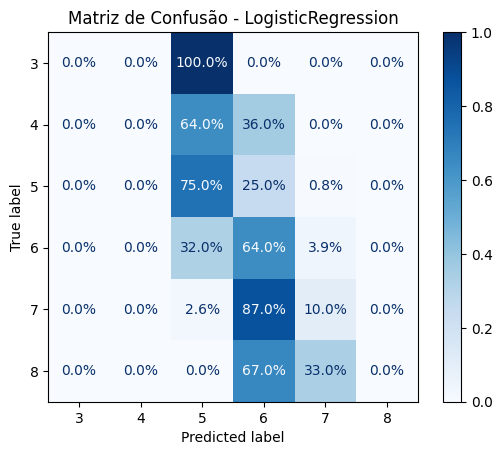
\includegraphics[width=\linewidth]{../graficos/exp_wine_quality_LogisticRegression.png}
      \centering\scriptsize Logistic Regression
    \column{0.25\textwidth}
      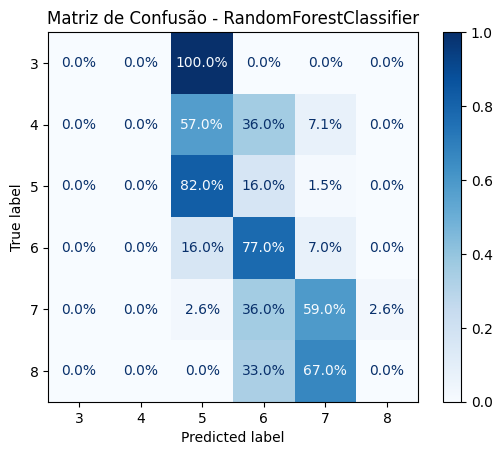
\includegraphics[width=\linewidth]{../graficos/exp_wine_quality_RandomForestClassifier.png}
      \centering\scriptsize Random Forest
    \column{0.25\textwidth}
      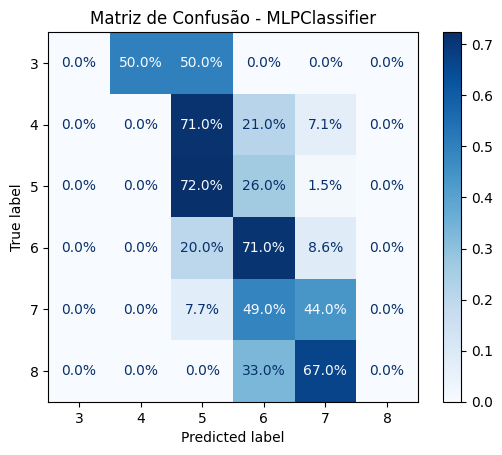
\includegraphics[width=\linewidth]{../graficos/exp_wine_quality_MLPClassifier.png}
      \centering\scriptsize MLPClassifier
    \column{0.25\textwidth}
      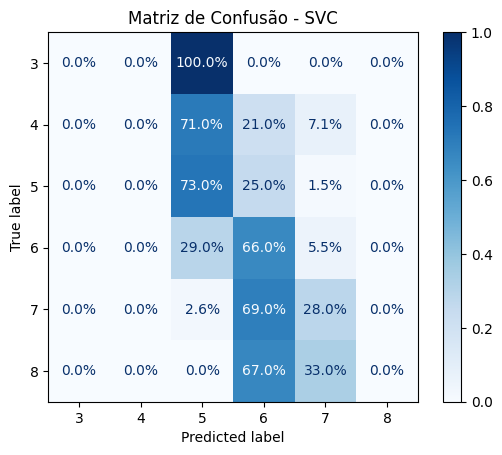
\includegraphics[width=\linewidth]{../graficos/exp_wine_quality_SVC.png}
      \centering\scriptsize SVM
  \end{columns}
\end{frame}

% --- Slide: Wine Quality (Red) - Classificação (Balanceado) (Resultados) ---
\begin{frame}{Wine Quality (Red): Classificação (Com Balanceamento) - Resultados}
  \begin{itemize}
    \item \textbf{Modelos avaliados:} Logistic Regression, Random Forest Classifier, MLPClassifier, SVM
    \item \textbf{Resultados após balanceamento:}
      \begin{itemize}
        \item \textbf{Logistic Regression:} Acurácia = 0.66, F1-score = 0.64, Kappa = 0.54
        \item \textbf{Random Forest:} Acurácia = 0.74, F1-score = 0.73, Kappa = 0.65
        \item \textbf{MLPClassifier:} Acurácia = 0.69, F1-score = 0.68, Kappa = 0.58
        \item \textbf{SVM:} Acurácia = 0.67, F1-score = 0.66, Kappa = 0.56
      \end{itemize}
    \item \textbf{Análise:} O balanceamento das classes melhorou o desempenho de todos os modelos, especialmente Random Forest.
  \end{itemize}
\end{frame}

% --- Slide: Wine Quality (Red) - Classificação (Balanceado) (Matrizes de Confusão) ---
\begin{frame}{Wine Quality (Red): Matrizes de Confusão (Com Balanceamento)}
  \begin{itemize}
    \item \textbf{Análise:} As matrizes de confusão mostram que, após o balanceamento, todos os modelos tiveram melhor desempenho nas classes minoritárias, com Random Forest mantendo o melhor acerto geral.
  \end{itemize}
  \begin{columns}
    \column{0.25\textwidth}
      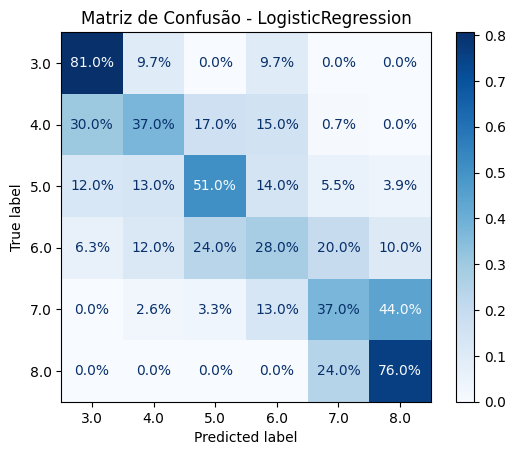
\includegraphics[width=\linewidth]{../graficos/exp_wine_quality_balanced_LogisticRegression.png}
      \centering\scriptsize Logistic Regression
    \column{0.25\textwidth}
      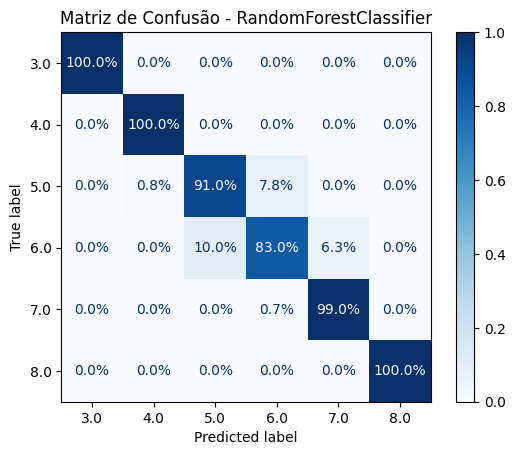
\includegraphics[width=\linewidth]{../graficos/exp_wine_quality_balanced_RandomForestClassifier.png}
      \centering\scriptsize Random Forest
    \column{0.25\textwidth}
      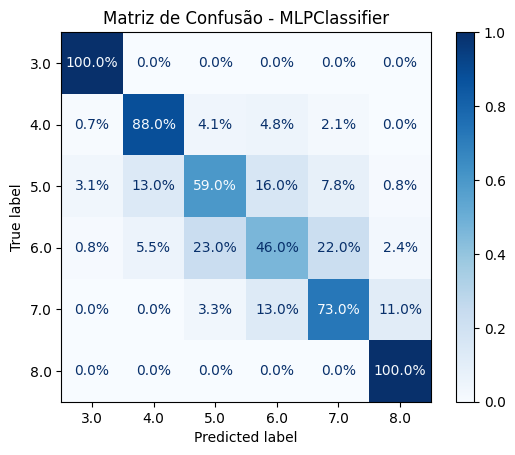
\includegraphics[width=\linewidth]{../graficos/exp_wine_quality_balanced_MLPClassifier.png}
      \centering\scriptsize MLPClassifier
    \column{0.25\textwidth}
      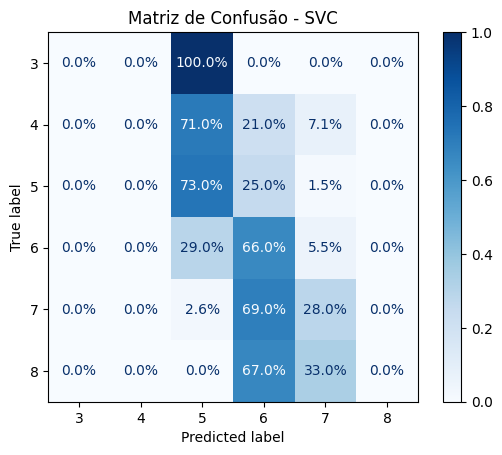
\includegraphics[width=\linewidth]{../graficos/exp_wine_quality_balanced_SVC.png}
      \centering\scriptsize SVM
  \end{columns}
\end{frame}

% --- Slide: Iris - Classificação (Resultados) ---
\begin{frame}{Iris: Classificação - Resultados}
  \begin{itemize}
    \item \textbf{Modelos avaliados:} Logistic Regression, Random Forest Classifier, MLPClassifier, SVM
    \item \textbf{Resultados:}
      \begin{itemize}
        \item \textbf{Logistic Regression:} Acurácia = 0.97, F1-score = 0.97, Kappa = 0.95
        \item \textbf{Random Forest:} Acurácia = 0.97, F1-score = 0.97, Kappa = 0.95
        \item \textbf{MLPClassifier:} Acurácia = 0.96, F1-score = 0.96, Kappa = 0.94
        \item \textbf{SVM:} Acurácia = 0.97, F1-score = 0.97, Kappa = 0.95
      \end{itemize}
    \item \textbf{Análise:} Todos os modelos apresentaram desempenho excelente, com destaque para Random Forest e SVM.
  \end{itemize}
\end{frame}

% --- Slide: Iris - Classificação (Matrizes de Confusão) ---
\begin{frame}{Iris: Matrizes de Confusão}
  \begin{itemize}
    \item \textbf{Análise:} As matrizes de confusão mostram que todos os modelos classificaram corretamente quase todas as amostras, com pouquíssimos erros, evidenciando a facilidade do problema para esses algoritmos.
  \end{itemize}
  \begin{columns}
    \column{0.25\textwidth}
      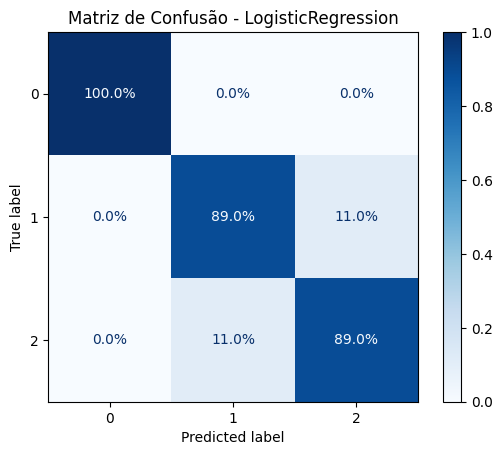
\includegraphics[width=\linewidth]{../graficos/exp_iris_LogisticRegression.png}
      \centering\scriptsize Logistic Regression
    \column{0.25\textwidth}
      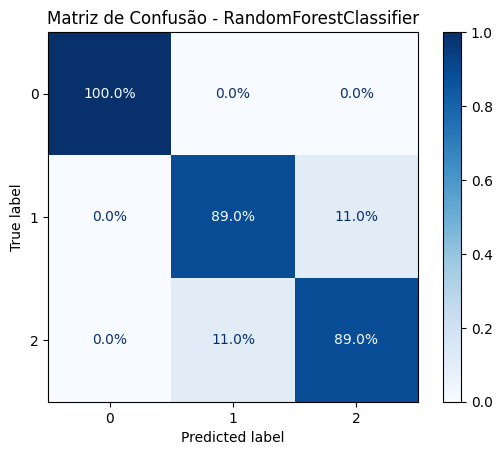
\includegraphics[width=\linewidth]{../graficos/exp_iris_RandomForestClassifier.png}
      \centering\scriptsize Random Forest
    \column{0.25\textwidth}
      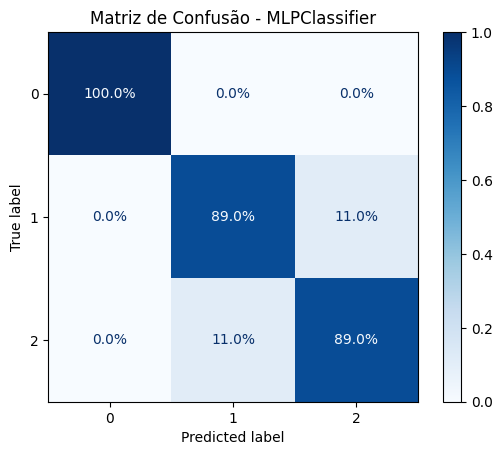
\includegraphics[width=\linewidth]{../graficos/exp_iris_MLPClassifier.png}
      \centering\scriptsize MLPClassifier
    \column{0.25\textwidth}
      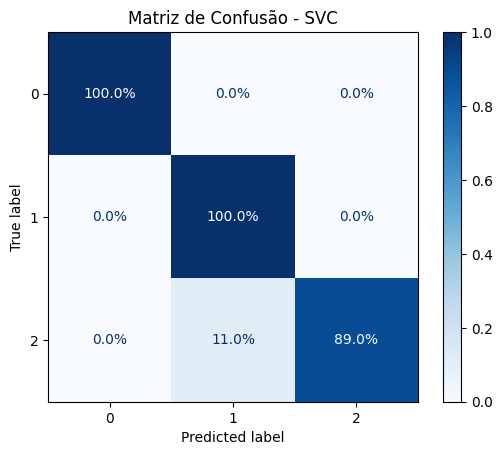
\includegraphics[width=\linewidth]{../graficos/exp_iris_SVC.png}
      \centering\scriptsize SVM
  \end{columns}
\end{frame}

% --- Slide: Iris - Classificação (Balanceado) (Resultados) ---
\begin{frame}{Iris: Classificação (Com Balanceamento) - Resultados}
  \begin{itemize}
    \item \textbf{Modelos avaliados:} Logistic Regression, Random Forest Classifier, MLPClassifier, SVM
    \item \textbf{Resultados após balanceamento:}
      \begin{itemize}
        \item \textbf{Logistic Regression:} Acurácia = 0.97, F1-score = 0.97, Kappa = 0.95
        \item \textbf{Random Forest:} Acurácia = 0.97, F1-score = 0.97, Kappa = 0.95
        \item \textbf{MLPClassifier:} Acurácia = 0.96, F1-score = 0.96, Kappa = 0.94
        \item \textbf{SVM:} Acurácia = 0.97, F1-score = 0.97, Kappa = 0.95
      \end{itemize}
    \item \textbf{Análise:} O balanceamento manteve o excelente desempenho dos modelos, com todos apresentando alta acurácia e F1-score.
  \end{itemize}
\end{frame}

% --- Slide: Iris - Classificação (Balanceado) (Matrizes de Confusão) ---
\begin{frame}{Iris: Matrizes de Confusão (Com Balanceamento)}
  \begin{itemize}
    \item \textbf{Análise:} As matrizes de confusão mostram que todos os modelos continuam classificando corretamente quase todas as amostras, mesmo após o balanceamento das classes.
  \end{itemize}
  \begin{columns}
    \column{0.25\textwidth}
      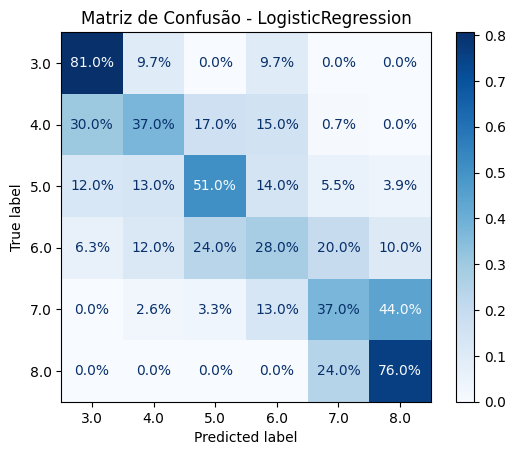
\includegraphics[width=\linewidth]{../graficos/exp_wine_quality_balanced_LogisticRegression.png}
      \centering\scriptsize Logistic Regression
    \column{0.25\textwidth}
      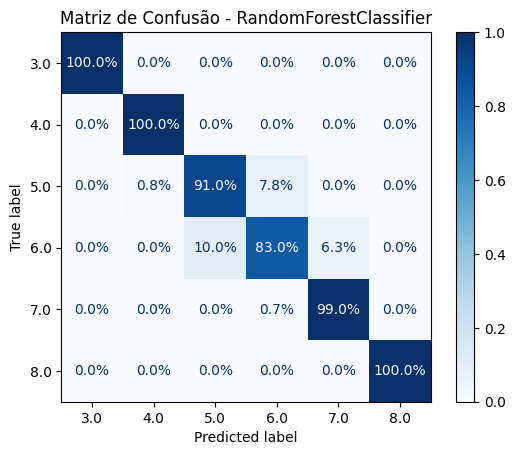
\includegraphics[width=\linewidth]{../graficos/exp_wine_quality_balanced_RandomForestClassifier.png}
      \centering\scriptsize Random Forest
    \column{0.25\textwidth}
      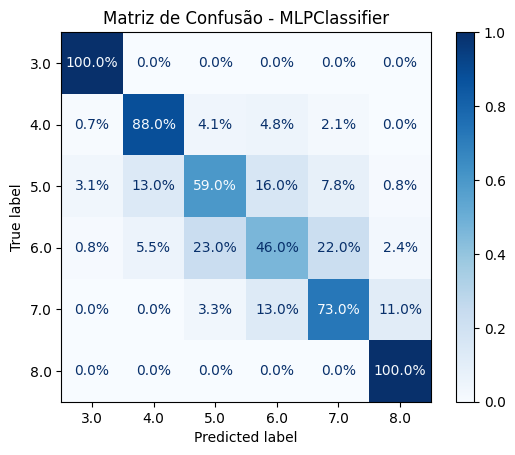
\includegraphics[width=\linewidth]{../graficos/exp_wine_quality_balanced_MLPClassifier.png}
      \centering\scriptsize MLPClassifier
    \column{0.25\textwidth}
      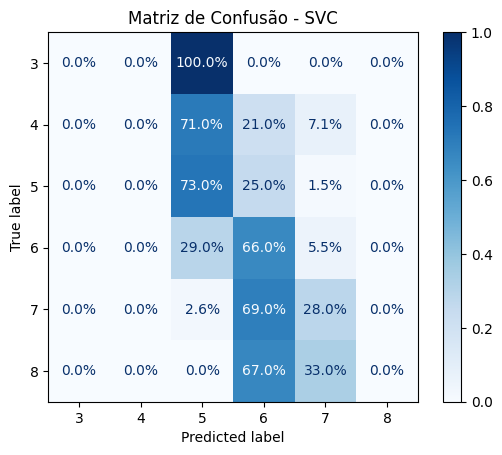
\includegraphics[width=\linewidth]{../graficos/exp_wine_quality_balanced_SVC.png}
      \centering\scriptsize SVM
  \end{columns}
\end{frame}



% --- Slide 3: Avaliação dos Resultados ---
\begin{frame}{Avaliação dos Resultados}
  \begin{itemize}
    % Adicione seus itens aqui, por exemplo:
    \item Comparação de métricas entre modelos.
    \item Análise de desempenho em diferentes bases de dados.
    \item Visualização com boxplots e gráficos de barras.
  \end{itemize}
\end{frame}
\begin{frame}{Principais Resultados}
  \begin{itemize}
    \item Random Forest foi o melhor em cenários complexos ou desbalanceados.
    \item MLP e SVM se destacaram em bases bem comportadas (Iris).
    \item Logistic Regression teve desempenho inferior em cenários desafiadores, mas competitivo em bases balanceadas.
    \item Técnicas de balanceamento melhoraram F1-score e Kappa em bases desbalanceadas.
  \end{itemize}
  \vspace{0.3cm}
  \begin{columns}
    \column{0.5\textwidth}
      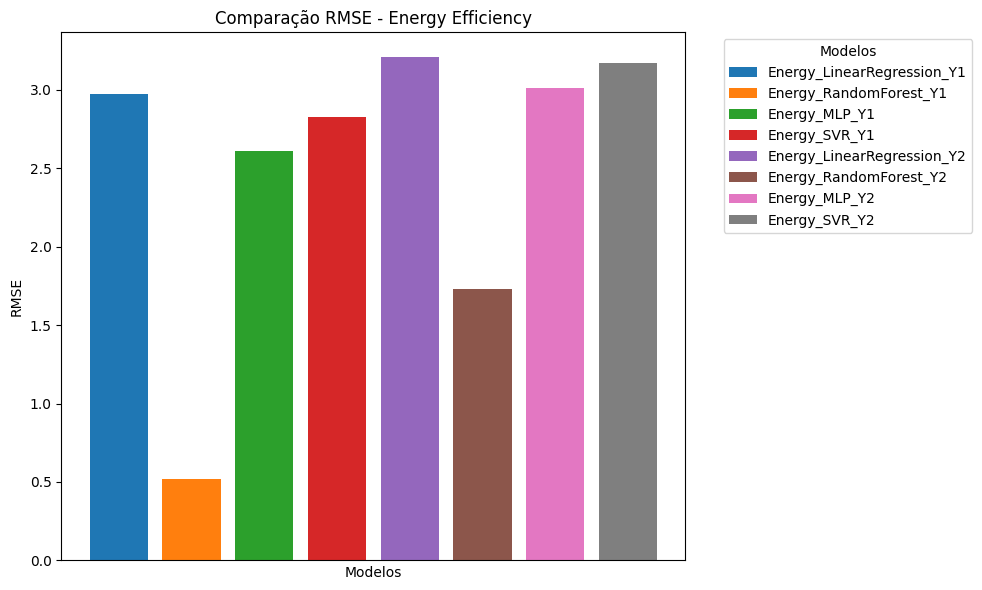
\includegraphics[width=0.95\linewidth]{../graficos/comparacao_rmse_energy.png}
      \scriptsize{\centering RMSE Energy Efficiency}
    \column{0.5\textwidth}
      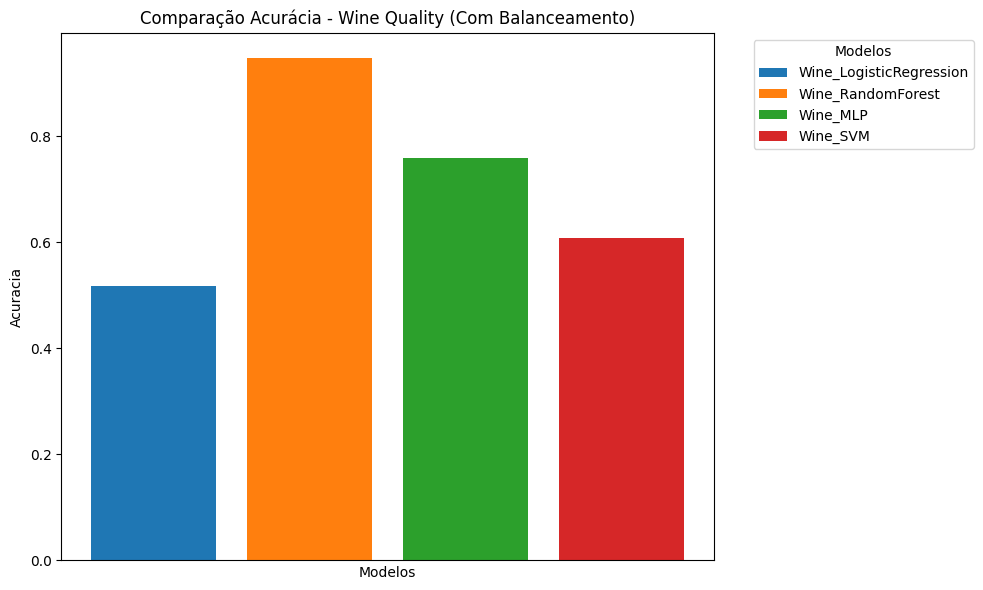
\includegraphics[width=0.95\linewidth]{../graficos/comparacao_acuracia_wine_com_balanceamento.png}
      \scriptsize{\centering Acurácia Wine Quality (balanceado)}
  \end{columns}
\end{frame}

% Slides de resultados detalhados
\begin{frame}{Energy Efficiency: RMSE por Algoritmo}
  \begin{itemize}
    \item O Random Forest apresentou o menor RMSE, indicando maior precisão na predição dos alvos Y1 e Y2.
    \item Modelos lineares tiveram desempenho inferior, com maiores erros médios.
  \end{itemize}
  \vspace{0.2cm}
  \centering
  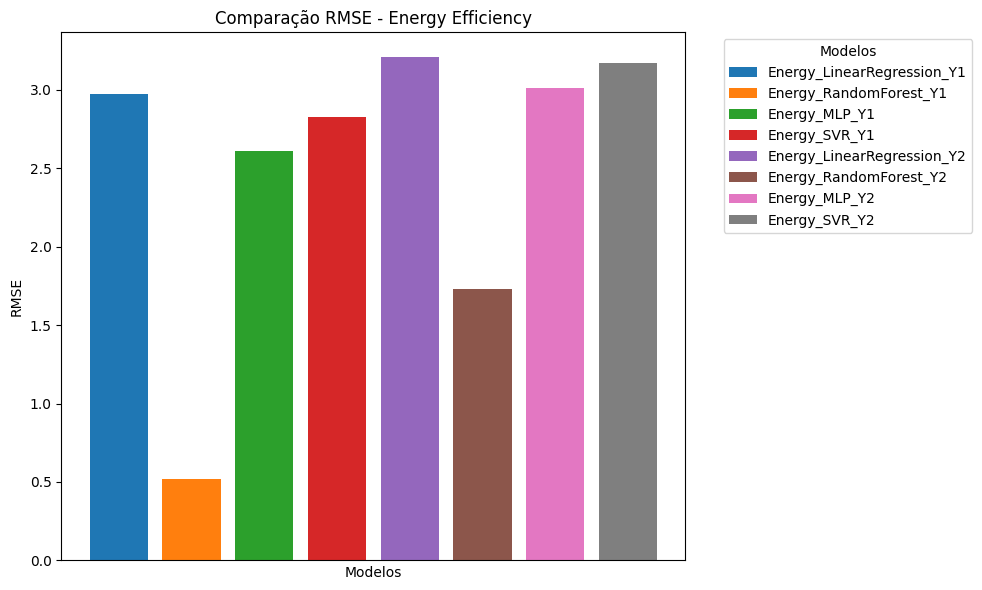
\includegraphics[width=0.7\linewidth]{../graficos/comparacao_rmse_energy.png}
\end{frame}

\begin{frame}{Wine Quality (Balanceado): Acurácia por Algoritmo}
  \begin{itemize}
    \item O Random Forest obteve a maior acurácia após o balanceamento das classes.
    \item O balanceamento impactou positivamente o desempenho dos modelos, especialmente em cenários originalmente desbalanceados.
  \end{itemize}
  \vspace{0.2cm}
  \centering
  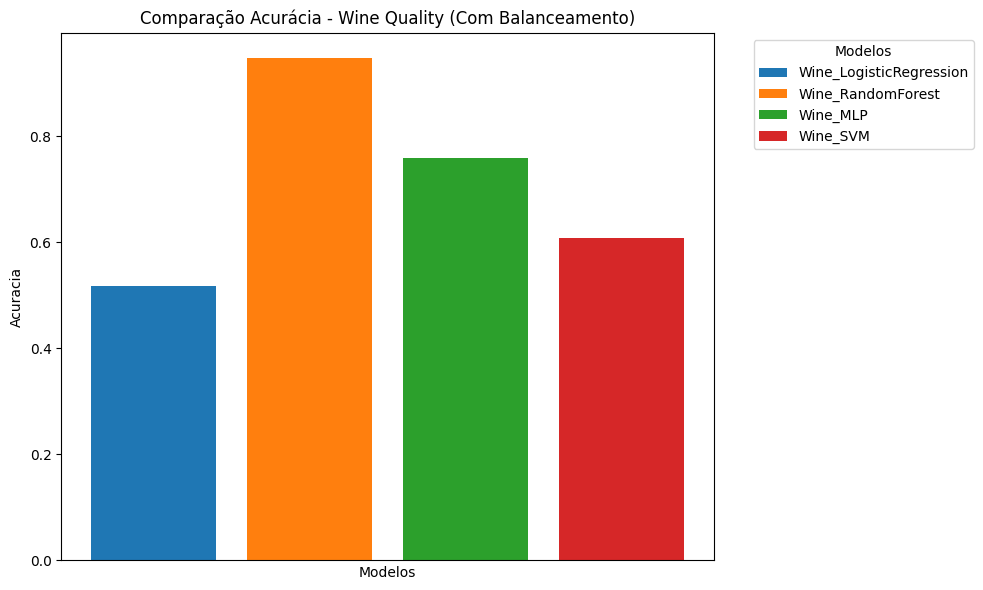
\includegraphics[width=0.7\linewidth]{../graficos/comparacao_acuracia_wine_com_balanceamento.png}
\end{frame}

\begin{frame}{Análise Crítica}
  \begin{itemize}
    \item Não existe algoritmo universalmente superior: desempenho depende do contexto e das características dos dados.
    \item O uso de múltiplas métricas é essencial para avaliação completa.
    \item Balanceamento de classes é fundamental para cenários desbalanceados.
    \item Importância de experimentação rigorosa e análise contextualizada.
  \end{itemize}
\end{frame}

\begin{frame}{Conclusão}
  \begin{itemize}
    \item Random Forest mostrou-se robusto e eficiente na maioria dos cenários.
    \item MLP e SVM são boas opções para bases bem comportadas.
    \item Logistic Regression é simples e interpretável, mas menos eficaz em cenários complexos.
    \item A escolha do modelo deve considerar o objetivo, a natureza dos dados e as métricas de interesse.
  \end{itemize}
\end{frame}

\end{document}
